% Chapter Template

\chapter{Data} % Main chapter title

\label{Chapter3} % Change X to a consecutive number; for referencing this chapter elsewhere, use \ref{ChapterX}

%----------------------------------------------------------------------------------------
%	SECTION 1
%----------------------------------------------------------------------------------------

\section{Dataset}

The dataset used to train and test the machine learning model was obtained from another paper that was working on a similar project. The authors of that paper made their dataset available online. There are 2252 songs in this dataset, 1802 of which had been categorised as the training set while the rest had been categorised as the test set. Each song is in major key and only have a single chord per bar. For each song, all the relevant features had been extracted and placed into a single \emph{CSV} file. These files can then be read and converted to DataFrame format using Python \emph{Pandas} as shown in Figure \ref{fig:CSV_DF}.

As can be seen in Figure \ref{fig:CSV_DF}, the rows each contain information about a single note. Each bar is taken to be a single measure. The columns each represent a different piece of information about that particular note. \emph{time} refers to the time signature, \emph{measure} refers to the measure to which that particular note belongs to, \emph{key\_fifths} indicates the number of sharps/flats (e.g. -1 for one flat and 1 for one sharp), \emph{chord\_root} is the root of the chord with \emph{chord\_type} indicating the type of chord, \emph{note\_root} identifies the particular single note of that row, \emph{note\_octave} is the octave of that note, and \emph{note\_duration} indicated the duration of the note (4.0 for a quarter note).

\begin{figure}
\centering
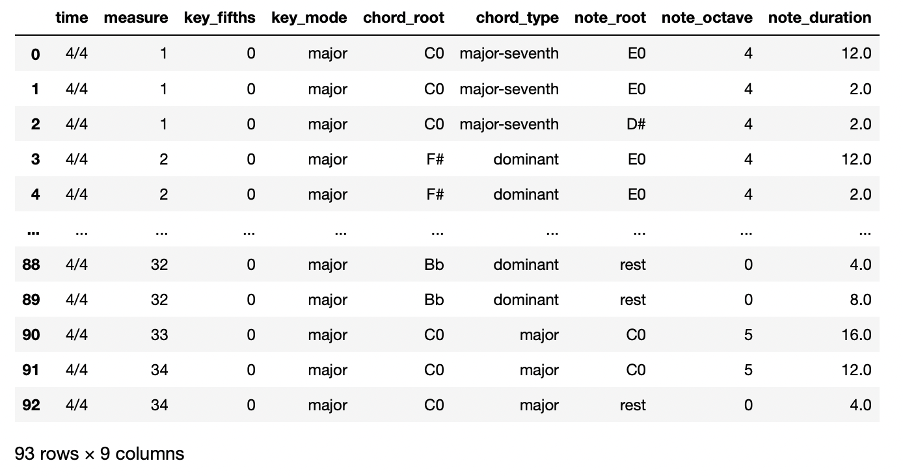
\includegraphics{Figures/CSV dataframe}
\decoRule
\caption{A song in DataFrame format after being read from CSV file}
\label{fig:CSV_DF}
\end{figure}

%-----------------------------------
%	SECTION 2
%-----------------------------------
\section{Preprocessing of dataset}

The dataset has to be preprocessed in order to make things simpler later on.

\begin{enumerate}
  \item All songs are transposed to C major key. The key of a song determines the notes and the set of chords present in the song. Transposing all songs to a common key will basically normalise the different features of melodies and chords in different songs. The number of chord types present in the dataset will be reduced, which will decrease the number of chord types during the training process. Each song can be shifted to a different key without loss of the song's subjective character by shifting all the pitches equally.
  \item The time signatures are all normalised. Different songs have different time signatures. To do so, each \emph{note\_duration} is multiplied by the reciprocal of the time signature \emph{time} to give a normalised note duration.
  \item Chord types are restricted to C major and C minor chords. All other chord types are converted to their most similar scale tone chords in key C.
  \item Some measures in the dataset contain rest notes. These measures are removed from the dataset.
  \item Octave information is not required and is removed from the dataset.
  \item There are also some irregular notes present in the dataset such as 'B-2' and 'A2'. The numbers after the letters do not seem to represent octave information and the paper from which this dataset was obtained made no mention of them. Given that they represent a very small portion of the dataset, measures containing these irregular notes are also removed.
\end{enumerate}

%-----------------------------------
%	SUBSECTION 1
%-----------------------------------
\subsection{Code}
Using \emph{Pandas} to remove the unwanted measures mentioned above and to normalise the note durations is a straightforward task. However, shifting all the songs to C major key is trickier. We would need to know the original key of the song, and then transposed the \emph{note\_root} and \emph{chord\_root} appropriately to C major key. The original keys of the songs are stated implicitly by their \emph{key\_fifths}; since we know all the songs are in major key and that each major key has a unique number of sharps/flats, the numberical value of \emph{key\_fifths} can be mapped to a specific major key as shown in Table \ref{tab:kf_map}. Note that there exist more values of \emph{key\_fifths} than shown, but preliminary analysis of the dataset shows that only integer values of \emph{key\_fifths} from -6 to 7 are present within it. We also create a mapping of the 12 notes to a numerical representation as shown in Table \ref{tab:note_map} to make the processing easier later.

Using Table \ref{tab:kf_map} \& \ref{tab:note_map}, we can list all the major keys present in the dataset and convert the pitches that exist within each major key into their numerical representations as shown in Table \ref{tab:bigtable}. As expected, the differences between the pitches of the same key are consistent across all the major keys (e.g. the difference between Pitch 1 and Pitch 3 is always 4 for every major key), which shows that we can indeed tranpose a song to a different key by just shifting all the pitches equally. For each DataFrame row, we just have to convert \emph{key\_fifths} to the corresponding major key using \ref{tab:kf_map} to obtain the numerical representaion of Pitch 1 of that major key. We also convert \emph{note\_root} and \emph{chord\_root} to numbers using Table \ref{tab:note_map}. Next, the numerical representation of Pitch 1 is subtracted from those of \emph{note\_root} and \emph{chord\_root}, and the differences are added to Pitch 1 of the C major key (which is 1) to obtain the shifted pitches in notes and chords respectively. Note that the differences may be negative, which would lead to a shifted note/chord that is outside of the 1-12 range. This is easily rectified by using \emph{if} statements to check if the shifted note/chord is non-positive and to add 12 (since a zero would loop back to 12) to it if so.
%\begin{figure}
 %   \centering
  %  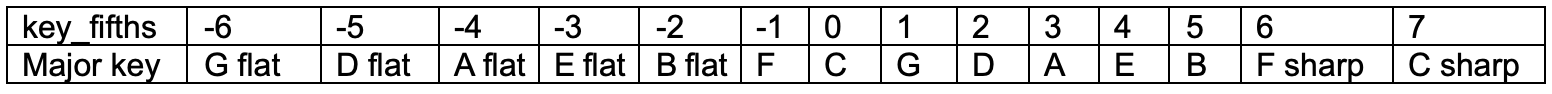
\includegraphics{Figures/key_fifths_mapping}
   % \decoRule
   % \caption{Mapping of \emph{key\_fifths} to major key}
   % \label{fig:kf_map}
    %\end{figure}

    \begin{table}
        \caption{Mapping of \emph{key\_fifths} to major key}
        \label{tab:kf_map}
        \centering
        \begin{tabular}{|c||c|c|c|c|c|c|c|c|c|c|c|c|c|c|}
        \hline
        \emph{key\_fifths} & -6 & -5 & -4 & -3 & -2 & -1 & 0 & 1 & 2 & 3 & 4 & 5 & 6 & 7 \\
        \hline
        Major key & Gb & Db & Ab & Eb & Bb & F & C & G & D & A & E & B & F\# & C\# \\
        \hline
        \end{tabular}
        \end{table}

\begin{table}
    \caption{Mapping of music notes to numerical representations}
    \label{tab:note_map}
    \centering
    \begin{tabular}{|c|c|c|c|c|c|}
    \hline
    C/B\# & C\#/Db & D & D\#/Eb & E/Fb & F/E\# \\
    \hline
    1 & 2 & 3 & 4 & 5 & 6 \\
    \hline
    \end{tabular}
    \begin{tabular}{|c|c|c|c|c|c|}
        \hline
    F\#/Gb & G & G\#/Ab & A & A\#/Bb & B/Cb\\
    \hline
    7 & 8 & 9 & 10 & 11 & 12\\
    \hline
    \end{tabular}
    \end{table}

    \begin{table}
        \caption{The component notes/pitches of each major key}
        \label{tab:bigtable}
        \centering
        \begin{tabular}{|c||c|c|c|c|c|c|c|}
        \hline
        Major key & Pitch 1 & Pitch 2 & Pitch 3 & Pitch 4 & Pitch 5 & Pitch 6 & Pitch 7 \\
        \hline
        \hline
        C\# & 2 & 4 & 6 & 7 & 9 & 11 & 1 \\
        \hline
        F\# & 7 & 9 & 11 & 12 & 2 & 4 & 6\\
        \hline
        B & 12 & 2 & 4 & 5 & 7 & 9 & 11\\
        \hline
        E & 5 & 7 & 9 & 10 & 12 & 2 & 4\\
        \hline
        A & 10 & 12 & 2 & 3 & 5 & 7 & 9\\
        \hline
        D & 3 & 5 & 7 & 8 & 10 & 12 & 2\\
        \hline
        G & 8 & 10 & 12 & 1 & 3 & 5 & 7\\
        \hline
        C & 1 & 3 & 5 & 6 & 8 & 10 & 12\\
        \hline
        F & 6 & 8 & 10 & 11 & 1 & 3 & 5\\
        \hline
        Bb & 11 & 1 & 3 & 4 & 6 & 8 & 10\\
        \hline
        Eb & 4 & 6 & 8 & 9 & 11 & 1 & 3\\
        \hline
        Ab & 9 & 11 & 1 & 2 & 4 & 6 & 8\\
        \hline
        Db & 2 & 4 & 6 & 7 & 9 & 11 & 1\\
        \hline
        Gb & 7 & 9 & 11 & 12 & 2 & 4 & 6\\
        \hline
        \end{tabular}
        \end{table}

        \begin{figure}
            \centering
            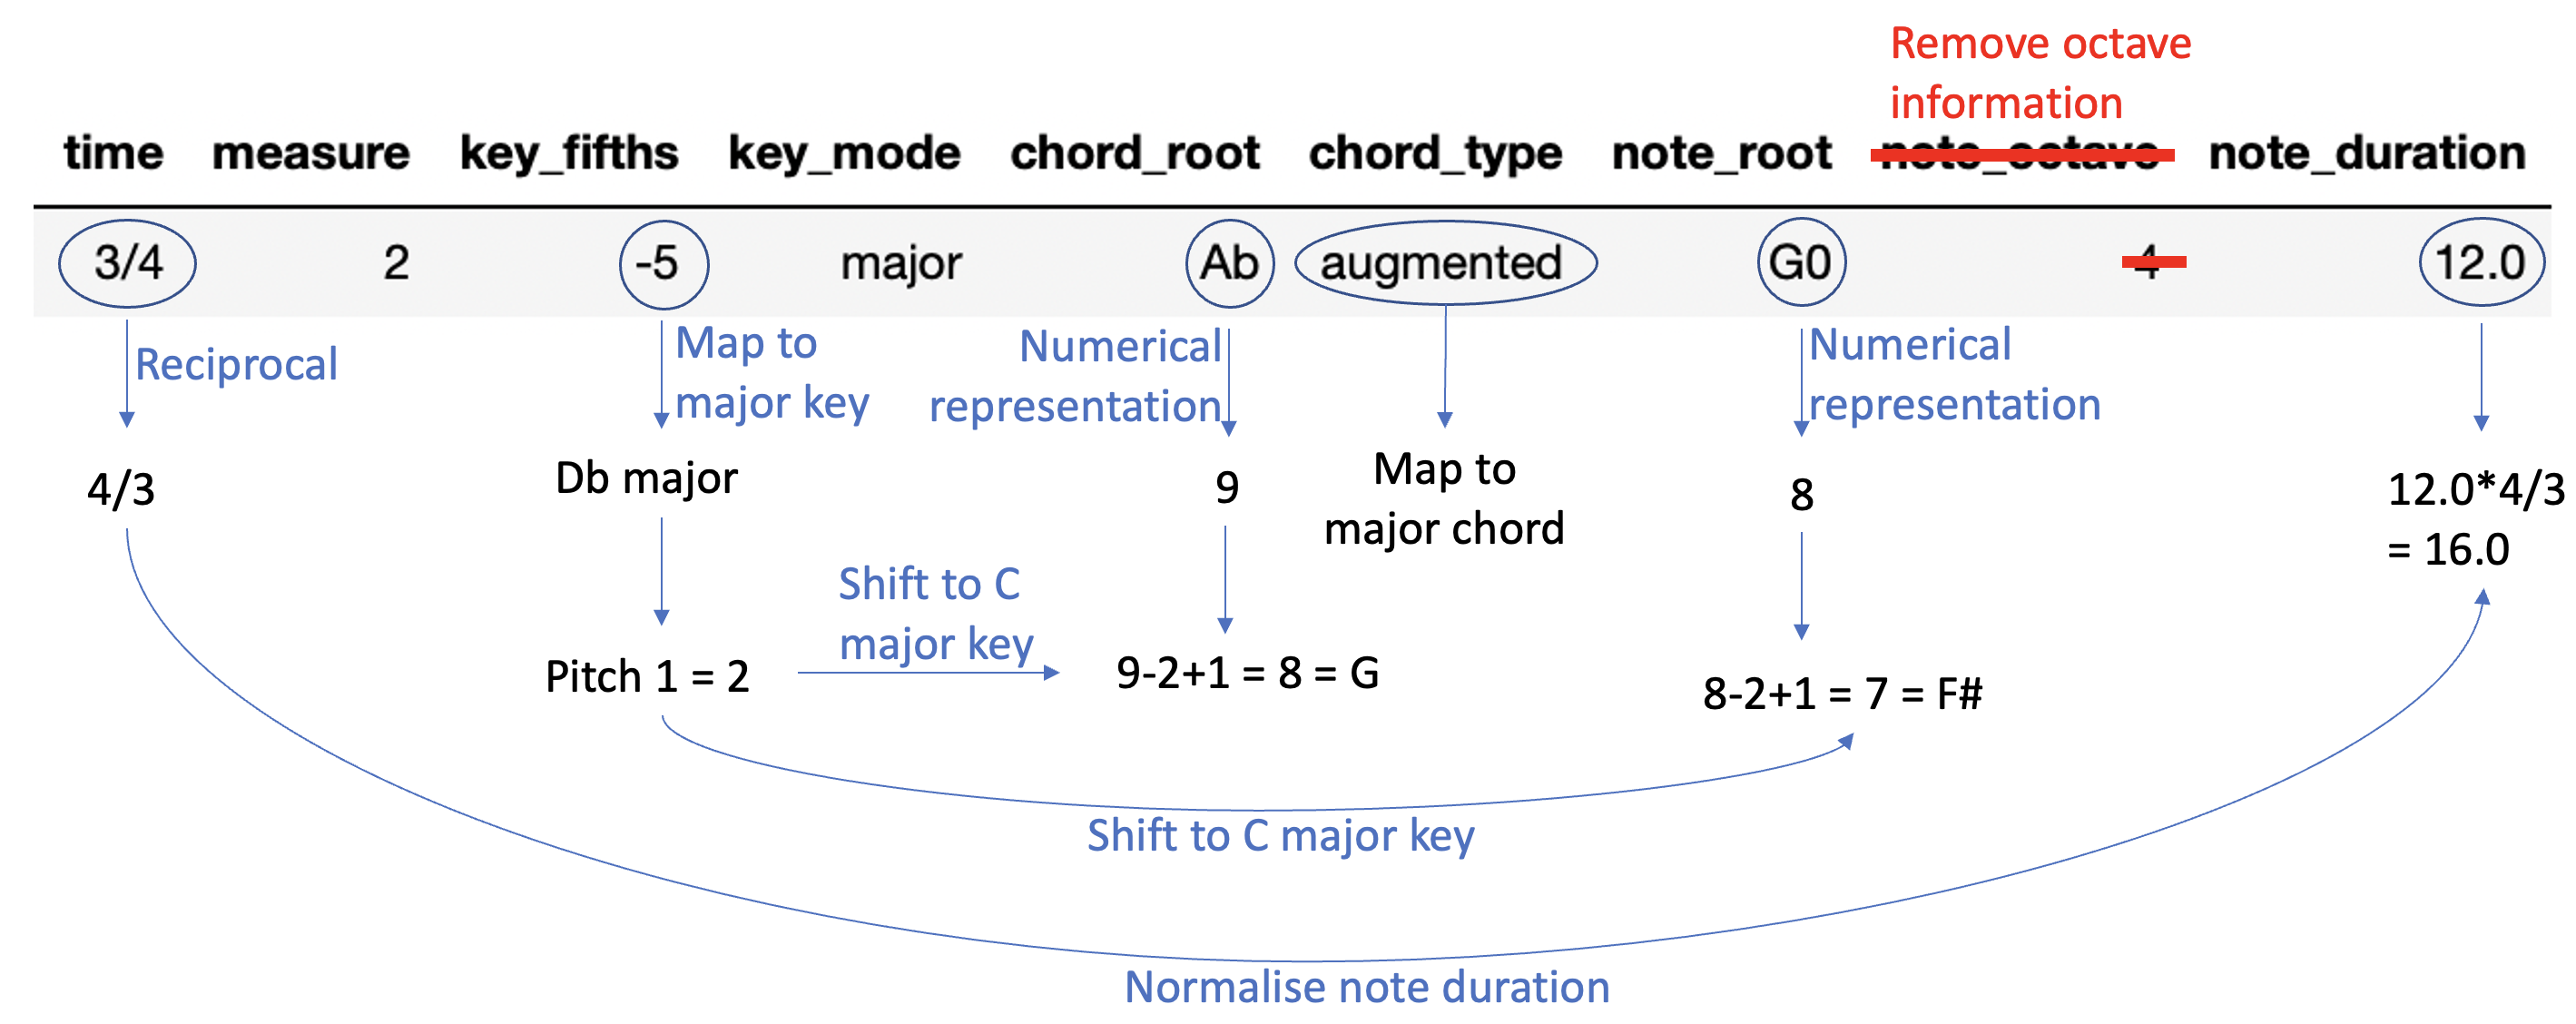
\includegraphics[scale=0.3]{Figures/Algorithm pictorial2}
            \decoRule
            \caption{Pictorial representation of the preprocessing of the dataset.}
            \label{fig:Alg1}
            \end{figure}
            
%-----------------------------------
%	SUBSECTION 2
%-----------------------------------

\subsection{Subsection 2}
Morbi rutrum odio eget arcu adipiscing sodales. Aenean et purus a est pulvinar pellentesque. Cras in elit neque, quis varius elit. Phasellus fringilla, nibh eu tempus venenatis, dolor elit posuere quam, quis adipiscing urna leo nec orci. Sed nec nulla auctor odio aliquet consequat. Ut nec nulla in ante ullamcorper aliquam at sed dolor. Phasellus fermentum magna in augue gravida cursus. Cras sed pretium lorem. Pellentesque eget ornare odio. Proin accumsan, massa viverra cursus pharetra, ipsum nisi lobortis velit, a malesuada dolor lorem eu neque.

%----------------------------------------------------------------------------------------
%	SECTION 2
%----------------------------------------------------------------------------------------

\section{Main Section 2}

Sed ullamcorper quam eu nisl interdum at interdum enim egestas. Aliquam placerat justo sed lectus lobortis ut porta nisl porttitor. Vestibulum mi dolor, lacinia molestie gravida at, tempus vitae ligula. Donec eget quam sapien, in viverra eros. Donec pellentesque justo a massa fringilla non vestibulum metus vestibulum. Vestibulum in orci quis felis tempor lacinia. Vivamus ornare ultrices facilisis. Ut hendrerit volutpat vulputate. Morbi condimentum venenatis augue, id porta ipsum vulputate in. Curabitur luctus tempus justo. Vestibulum risus lectus, adipiscing nec condimentum quis, condimentum nec nisl. Aliquam dictum sagittis velit sed iaculis. Morbi tristique augue sit amet nulla pulvinar id facilisis ligula mollis. Nam elit libero, tincidunt ut aliquam at, molestie in quam. Aenean rhoncus vehicula hendrerit.